%%      --- TO DO --- 
%%    Abstand des Chapters zu stark... --> ist aber kein Chapter design problem sondern randproblem allgemein
%%    Umbennenung des LHC Kapitels in Accelerator complex o.Ä.
\documentclass[pdftex, a4paper, parskip=full*, open=any, BCOR=10mm, fontsize=12pt, DIV=12, headsepline, footsepline=true, footinclude=false, draft=false, captions=nooneline]{scrbook}  %pdftex,
%
%\usepackage[utf8]{inputenc}
\usepackage[T1]{fontenc}
\usepackage{lmodern}
\usepackage{amsmath, amsthm, amssymb}
\usepackage{mathtools}
\usepackage{graphicx}
\usepackage{array}
\usepackage{babelbib}
\usepackage{verbatim}
\usepackage{lscape}
\usepackage{textcomp}    %fuer aufrechte mu
\usepackage[english]{babel}
\usepackage{caption}%Ist Voraussetzung für das Subcaption package, welches die subfigures erlaubt
\usepackage{subcaption}%Für Einbindung von Bildern als Untergraphiken subfig(ure) sind veraltet!
\renewcommand*{\chapterformat}{%Chapter Design
  \enskip\mbox{\scalebox{2}{\thechapter\autodot}}}
\renewcommand\chapterlinesformat[3]{%
  \parbox[b]{\textwidth}{\textcolor{royalazure}{\hrulefill#2}}\par%
  #3\par\bigskip%
  \textcolor{royalazure}{\hrule}}
\RedeclareSectionCommand[afterskip=1.5\baselineskip]{chapter}
%\usepackage[numbers]{natbib}
\usepackage{hyperref}
\usepackage{url}
%\usepackage{ziffer} %für Kommas bei Zahlen
\usepackage{multirow}
\usepackage[table]{xcolor}
%\usepackage{bibgerm}
%Aus dem Praktikum...
\usepackage{ae}                %macht schöneres ß
\usepackage[margin=10pt,font=small,labelfont=bf]{caption} %macht die Bildbeschriftungen richtig
\usepackage{epsfig}%Zur Einbindung von .eps: eps-->pdf
\usepackage{rotating}%für Querformat einer Tabelle 
\usepackage[binary-units=true]{siunitx} %SI unit package mit binary units = bits, bytes
%\renewcommand{\figurename}{Abb.}
\setlength\parindent{1em}%Rückt am Absatzbeginn ein
%......ENDE
\renewcommand{\thefootnote}{\fnsymbol{footnote}}%Symbole für Fußnoten und keine default arabics
\makeatletter%Clear counter nach jedem Kapitel für die Fußnoten
\@addtoreset{footnote}{section}% ""
\makeatother% ""
\addtokomafont{caption}{\small}
\setkomafont{captionlabel}{\bfseries \sffamily}
%\bibliographystyle{gerplain} %Ist jetzt im Hauptdokument verbaut-->s. \bibliography{}
\definecolor{royalazure}{rgb}{0.0, 0.22, 0.66}
\renewcommand*\chapterheadstartvskip{\vspace*{-\topskip}}%Seitenrandanfang einstellen
\renewcommand*\chapterheadendvskip{%Seitenrandende einstellen
  \vspace*{1\baselineskip plus .1\baselineskip minus .167\baselineskip}}

\newcommand{\ATLAS}{\textsc{atlas}}%for small capitals, looks even nicer
\newcommand{\CERN}{\textsc{cern}}
\newcommand{\LHC}{\textsc{lhc}}
\newcommand{\ALICE}{\textsc{alice}}
\newcommand{\CMS}{\textsc{cms}}
\newcommand{\LINAC}{\textsc{linac}}
\hyphenation{
  %Aus-gangs-sig-nal Be-trach-tet er-folg-reich Über-gangs-strah-lungs-de-tek-tor
}

% Keine "Schusterjungen"
	\clubpenalty = 9999
% Keine "Hurenkinder"
	\widowpenalty = 9999 \displaywidowpenalty = 9999

\begin{document}
\begin{titlepage}
  \vspace*{-7\baselineskip}
	\enlargethispage{100mm}
		\begin{center}
		\LARGE{\textbf{Master Thesis}\\}
		\vspace{3mm}	
		\textcolor{royalazure}{\noindent\rule{\textwidth}{3pt}}
		\huge{\textbf{Signal and background studies for scalar leptoquark pair production in the t$\bar{\textbf{t}}\,\mathbf{+\,2\tau}$ channel at the ATLAS experiment}\\}
		\vspace{3mm}
		\Large{Daniel Adlkofer\\}
		\textcolor{royalazure}{\noindent\rule{\textwidth}{3pt}}
		\vspace{3mm}
        
\includegraphics[width=0.55\textwidth]{figures/neuSIEGEL.eps} \\
		\vspace{3mm}
		Supervisor \\
		\Large{Prof. Dr. Raimund Str\"{o}hmer\\}
               	\vspace{3mm}
                Advisor \\
    \Large{Dr. Mahsana Haleem\\}
               	\vspace{3mm}

		\vspace{5mm}
		December 2018\\
		  \noindent\hrulefill\\
		\vspace{3mm}
 		Lehrstuhl f\"{u}r Physik und ihre Didaktik\\
 		Physikalisches Institut\\
	    Julius-Maximilians-Universit\"{a}t W\"{u}rzburg
	\end{center}
\end{titlepage}
\cleardoubleoddemptypage

\tableofcontents
%%%%%%%%%%%%%%%%%%%%%%%%%%%%%%%%%%%%%%%%%%%%%%%%%%%%%%%%%%%%%%%%%%%%%%%%%%%%%%%%%%%%%%%%%%%%%%%%%%%
\chapter{XyZ}
%%%%%%%%%%%%%%%%%%%%%%%%%%%%%%%%%%%%%%%%%%%%%%%%%%%%%%%%%%%%%%%%%%%%%%%%%%%%%%%%%%%%%%%%%%%%%%%%%%%
$\SI{2}{\electronvolt\per\meter}$
\begin{table}[htbp]
		\centering
		\begin{tabular*}{\linewidth}{@{\extracolsep{\fill}}ccccc}
		\hline
		\hline
		\rule[-6pt]{0pt}{21pt} \textbf{sample}  & \multicolumn{2}{c}{\textbf{t$\bar{\textbf{t}}$}}  & \multicolumn{2}{c}{\textbf{t$\bar{\textbf{t}}$H}} 
		\\
		\hline
		\rule[-7pt]{0pt}{23pt} \multirow{2}{*}{selection}  & reconstruction & truth & reconstruction & truth  
		\\ 
		\rule[-7pt]{0pt}{23pt}  & event yield & event yield & event yield & event yield 
		\\
		\hline
		\rule[-6pt]{0pt}{21pt} $\geq 2\,$b-jets   & $66878$ & $252200$ & $73$ & $200$
		\\
		\rule[-6pt]{0pt}{21pt} $\geq 2\,$b-jets $+1\,\tau$  & $188$ & $5923$ & $2.5$ & $28$
		\\
		\rule[-6pt]{0pt}{21pt} $\geq 2\,$b-jets $+2\,\tau$ & $0.7$ & $49$ & $0.2$ & $8.2$ 
		\\
		\hline
		\hline
		\end{tabular*}
		\caption[Event yield for the t$\bar{\text{t}}$ and the t$\bar{\text{t}}$H sample.]{Event yield for different selections with tau leptons for the t$\bar{\text{t}}$ and the t$\bar{\text{t}}$H Monte Carlo sample. The luminosity account for $36.1\,\text{fb}^{-1}$.}
		\label{ttHttbarEvent}
	\end{table}
%
\begin{table}[htbp]
		\centering
		\begin{tabular*}{\linewidth}{@{\extracolsep{\fill}}ccc}
		\hline
		\hline
		\rule[-6pt]{0pt}{21pt} \textbf{sample}  & \textbf{t$\bar{\textbf{t}}$} & \textbf{t$\bar{\textbf{t}}$H}
		\\
		\hline
		\rule[-7pt]{0pt}{23pt} selection  & efficiency $\frac{\epsilon}{\%}$ & efficiency $\frac{\epsilon}{\%}$ 
		\\
		\hline
		\rule[-6pt]{0pt}{21pt} $\geq 2\,$b-jets & $26.52$ & $36.72$ 
		\\
		\rule[-6pt]{0pt}{21pt} $\geq 2\,$b-jets $+1\,\tau$  & $3.18$ & $8.83$ 
		\\
		\rule[-6pt]{0pt}{21pt} $\geq 2\,$b-jets $+2\,\tau$  & $1.41$ & $2.13$ 
		\\
		\hline
		\hline
		\end{tabular*}
		\caption[Efficiencies for the t$\bar{\text{t}}$ and the t$\bar{\text{t}}$H sample.]{Efficiencies for different selections with tau leptons for the t$\bar{\text{t}}$ and the t$\bar{\text{t}}$H Monte Carlo sample.}
		\label{ttHttbarEff}
	\end{table}
%
%
%
%
\begin{table}[htbp]
		\centering
		\begin{tabular*}{\linewidth}{@{\extracolsep{\fill}}cccccc}
		\hline
		\hline
		\rule[-6pt]{0pt}{21pt} \textbf{sample} & & \multicolumn{2}{c}{\textbf{t$\bar{\textbf{t}}$}}  & \multicolumn{2}{c}{\textbf{t$\bar{\textbf{t}}$H}} 
		\\
		\hline
		\rule[-7pt]{0pt}{23pt} \multirow{2}{*}{selection} & reference & reconstruction & truth & reconstruction & truth  
		\\ 
		\rule[-7pt]{0pt}{23pt} & selection & ratio $\frac{r}{\%}$ & ratio $\frac{r}{\%}$ & ratio $\frac{r}{\%}$ & ratio $\frac{r}{\%}$ 
		\\
		\hline
		\rule[-6pt]{0pt}{21pt} $\geq 2\,$b-jets $+1\,\tau$ & $\geq 2\,$b-jets & $0.28$ & $2.35$ & $3.43$ & $14.26$
		\\
		\rule[-6pt]{0pt}{21pt} $\geq 2\,$b-jets $+2\,\tau$ & $\geq 2\,$b-jets & $0.0011$ & $0.020$ & $0.24$ & $4.11$ 
		\\
		\hline
		\hline
		\end{tabular*}
		\caption[Ratios for the t$\bar{\text{t}}$ and the t$\bar{\text{t}}$H sample.]{Ratios for different selections with tau leptons for the t$\bar{\text{t}}$ and the t$\bar{\text{t}}$H Monte Carlo sample.}
		\label{ttHttbarRatio}
	\end{table}
%	
%
%	
%	
	\begin{table}[htbp]
		\centering
		\begin{tabular*}{\linewidth}{@{\extracolsep{\fill}}ccccc}
		\hline
		\hline
		\rule[-6pt]{0pt}{21pt} \textbf{sample}  & \multicolumn{2}{c}{\textbf{t$\bar{\textbf{t}}$}}  & \multicolumn{2}{c}{\textbf{t$\bar{\textbf{t}}$H}} 
		\\
		\hline
		\rule[-7pt]{0pt}{23pt} \multirow{2}{*}{selection}  & numerator      & denominator & numerator      & denominator
		\\ 
		\rule[-7pt]{0pt}{23pt}                             & event yield    & event yield & event yield    & event yield 
		\\
		\hline
		\rule[-6pt]{0pt}{21pt} truth matching for tau      & $63$            & $13723$      & $5590$        & $21610$
		\\
		\rule[-6pt]{0pt}{21pt} efficiency                  & \multicolumn{2}{c}{$0.46\%$}    & \multicolumn{2}{c}{$25.9\%$}
		\\
		\hline
		\rule[-6pt]{0pt}{21pt} tau from H$^0$, W$^{\pm}$, Z$^0$& $0$        & $0$         & $4859$          & $11988$
		\\
		\rule[-6pt]{0pt}{21pt} efficiency                  & \multicolumn{2}{c}{-}   & \multicolumn{2}{c}{$40.5\%$}
		\\
		\hline
		\rule[-6pt]{0pt}{21pt} tau from B-mesons           & $63$            & $13722$      & $20$            & $7416$ 
		\\
		\rule[-6pt]{0pt}{21pt} efficiency                  & \multicolumn{2}{c}{$0.46\%$}   & \multicolumn{2}{c}{$0.27\%$}
		\\
		\hline
		\rule[-6pt]{0pt}{21pt} tau within a jet            & $8440$         & $3776952$      & $18511$         & $20327225$ 
		\\
		\rule[-6pt]{0pt}{21pt} efficiency                  & \multicolumn{2}{c}{$0.22\%$}   & \multicolumn{2}{c}{$0.091\%$}
		\\
		\hline
		\rule[-6pt]{0pt}{21pt} tau within a b-jet          & $6098$        & $2658379$      & $2317$         & $1208924$ 
		\\
		\rule[-6pt]{0pt}{21pt} efficiency                  & \multicolumn{2}{c}{$0.23\%$}   & \multicolumn{2}{c}{$0.19\%$}
		\\
		\hline
		\hline
		\end{tabular*}
		\caption[Event yield for the t$\bar{\text{t}}$ and the t$\bar{\text{t}}$H sample.]{Event yield for different selections with tau leptons for the t$\bar{\text{t}}$ and the t$\bar{\text{t}}$H Monte Carlo sample. The luminosity account for $36.1\,\text{fb}^{-1}$.}
		\label{ttHttbarEventTruthMatching}
	\end{table}
%
%
%
%
	\begin{table}[htbp]
		\centering
		\begin{tabular*}{\linewidth}{@{\extracolsep{\fill}}ccccc}
		\hline
		\hline
		\rule[-6pt]{0pt}{21pt} \textbf{sample}  & \multicolumn{2}{c}{LQ${_{\SI{500}{\giga\electronvolt}}}$}  & \multicolumn{2}{c}{LQ${_{\SI{1}{\tera\electronvolt}}}$} 
		\\
		\hline
		\rule[-7pt]{0pt}{23pt} \multirow{2}{*}{selection}  & numerator      & denominator & numerator      & denominator
		\\ 
		\rule[-7pt]{0pt}{23pt}                             & event yield    & event yield & event yield    & event yield 
		\\
		\hline
		\rule[-6pt]{0pt}{21pt} truth matching for tau      & $2604$            & $5362$      & $2263$        & $5055$
		\\
		\rule[-6pt]{0pt}{21pt} efficiency                  & \multicolumn{2}{c}{$48.6\%$}    & \multicolumn{2}{c}{$44.8\%$}
		\\
		\hline
		\rule[-6pt]{0pt}{21pt} tau from H$^0$, W$^{\pm}$, Z$^0$& $95$        & $340$         & $82$          & $461$
		\\
		\rule[-6pt]{0pt}{21pt} efficiency                  & \multicolumn{2}{c}{$27.9\%$}   & \multicolumn{2}{c}{$17.8\%$}
		\\
		\hline
		\rule[-6pt]{0pt}{21pt} tau from B-mesons           & $0$            & $183$      & $0$            & $200$ 
		\\
		\rule[-6pt]{0pt}{21pt} efficiency                  & \multicolumn{2}{c}{$0.0\%$}   & \multicolumn{2}{c}{$0.0\%$}
		\\
		\hline
		\rule[-6pt]{0pt}{21pt} tau from LQ                 & $1744$            & $3286$      & $1057$            & $2022$ 
		\\
		\rule[-6pt]{0pt}{21pt} efficiency                  & \multicolumn{2}{c}{$53.1\%$}   & \multicolumn{2}{c}{$52.3\%$}
		\\
		\hline
		\rule[-6pt]{0pt}{21pt} tau within a jet            & $7232$         & $55208$      & $7011$         & $63671$ 
		\\
		\rule[-6pt]{0pt}{21pt} efficiency                  & \multicolumn{2}{c}{$13.1\%$}   & \multicolumn{2}{c}{$11.0\%$}
		\\
		\hline
		\rule[-6pt]{0pt}{21pt} tau within a b-jet          & $2317$        & $1208924$      & $6098$         & $2658379$ 
		\\
		\rule[-6pt]{0pt}{21pt} efficiency                  & \multicolumn{2}{c}{$0.45\%$}   & \multicolumn{2}{c}{$0.23\%$}
		\\
		\hline
		\hline
		\end{tabular*}
		\caption[]{}
		\label{LQEventTruthMatching}
	\end{table}
%%%%%%%%%%%%%%%%%%%%%%%%%%%%%%%%%%%%%%%%%%%%%%%%%%%%%%%%%%%%%%%%%%%%%%%%%%%%%%%%%%%%%%%%%%%%%%%%%%%%%%%%%%%%%%%%%%%%%%%%%%%
\chapter{Introduction}
%einen gescheiten Einleitungsgedanken überlegen! Ja nicht Higgs... :see_no_evil:
%Yukawa Kopplung vielleicht? --> ich bin mir nicht mehr sicher, aber vielleicht habe ich da einen Artikel gelesen (News CERN oder so) wo es um die noch bessere Messung der Yukawa Kopplung ging...
%%%%%%%%%%%%%%%%%%%%%%%%%%%%%%%%%%%%%%%%%%%%%%%%%%%%%%%%%%%%%%%%%%%%%%%%%%%%%%%%%%%%%%%%%%%%%%%%%%%%%%%%%%%%%%%%%%%%%%%%%%%%%
\chapter{Experimental setup for the search of scalar leptoquarks}\label{experiment}
For the search of scalar leptoquarks the ATLAS detector at the Large Hadron Collider (LHC) is used as experimental setup which will be described within this chapter. In section \ref{LHC} the general setting of the proton-proton collider located at the CERN research center is the subject of interest. The particle detection of the resulting collision events will take place in the ATLAS detector with its different specialized components (section \ref{ATLAS}). Section \ref{LQpp} addresses the leptoquark pair production in proton-proton collisions.  
\section{The Large Hadron Collider}\label{LHC}
The research center CERN (Conseil Européen pour la Recherche Nucléaire) was founded in $1954$ near Geneva, Switzerland to become a major European joint venture on elementary particle physics. In the mean time $22$ member states are participating in that large-scale project with the ambition to probe the essential constitutes of nature and the fundamental forces acting between them. \cite{CERNabout}\par
%
\begin{figure}[htbp]                                 
 \begin{center}                                       
  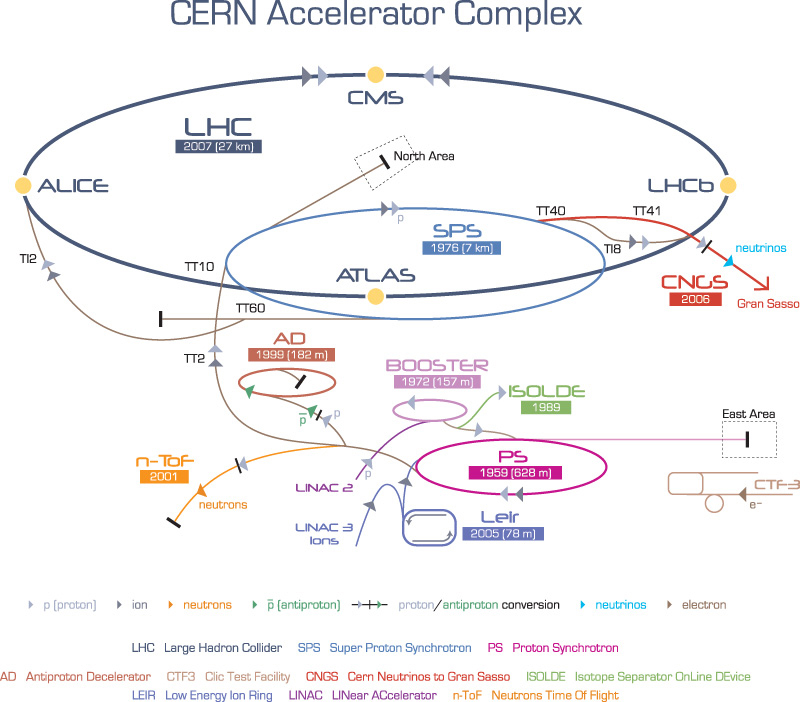
\includegraphics[width=0.55\linewidth]{figures/CERNKomplex.jpg} 
   \caption[Schematic of the CERN accelerator complex.]{Schematic of the CERN accelerator complex with its different stages and few experiments like ATLAS located at a crossing point for protons. \cite{CERNKomplex}}
  \label{complex}                                     
 \end{center}
\end{figure}
%
In the huge accelerator complex protons reach through different stages energies of $\SI{6.5}{\tera\electronvolt}$ and will be brought to collisions at defined interaction sites in time intervals of $\SI{25}{\nano\second}$. Particle detectors then register signatures of the resulting collsion events and the analysis of new created particles gives insight to the nature of elementary particle physics.\newline 
Figure \ref{complex} shows the different acceleration stages. Starting from the injection protons will gain as much energy as $\SI{50}{\mega\electronvolt}$ in the linear accelerator LINAC2 and will be further transferred to the Proton Synchrotron Booster ($\SI{1.4}{\giga\electronvolt}$), the Proton Synchrotron ($\SI{25}{\giga\electronvolt}$), the Super Proton Synchrotron ($\SI{450}{\giga\electronvolt}$) and finally to the LHC ring with its $\SI{26.7}{\kilo\meter}$ circumference. \cite{CERNabout}\newline
The LHC is designed as two-ring proton-proton collider. Conditions for a stable proton beam are diversely including high vacua of $\SI{E-10}{\milli\bar}$ to $\SI{E-11}{\milli\bar}$ and temperatures of $\SI{1.9}{\kelvin}$ for the superconducting NbTi-magnets of the accelerator. \cite{LHCJINST}   
%hier dann weiter ins Detail wie LHC JINST #######################
%Die Idee ist eigentlich eine genauere Beschreibung der Komponenten, allerdings ist JINST schon wieder so tief... So überblicksmäßiger wäre viel bessser, bei dem man noch im Blick behalten kann, um was es eigentlich geht...
\par
Different more experiments like ALICE\cite{ALICE}, LHCb\cite{LHCb} are located at CERN due to the variety of research questions. But the subject of interest in this work lies in the high luminosity experiment ATLAS specialized for proton-proton collisions like its counterpart CMS\cite{CMS}. 
%AußerdeM: Hinweis auf high Lumi LHC als Art mini-Ausblick in diesem Kapitel https://arxiv.org/pdf/1705.08830.pdf ################
%%%%%%%%%%%%%%%%%%%%%%%%%%%%%%%%%%%%%%%%%%%%%%%%%%%%%%%%%%%%%%%%%%%%%%%%%%%%%%%%%%%%%%%%%%%%%%%%%%%%%
\section{The ATLAS detector at the LHC}\label{ATLAS}
%Aufbau Idee: auch so ein Walktrough durch die einzelnen Komponenten wie bei der Bachelorarbeit
%Beschleunigungskette-->einzelne Komponenten + Trigger(ref auf Datenauswertung, Software part im Text dann)
%wahrscheinlich insgesamt genauer und etwas ausführlicher, da ein Schwerpunkt auf ein Detektorsystem keinen Sinn macht (schaue auch taus, jets, leptonen an...
%Motivation erher sogar von der Seite, wieso so gebaut, wie er ist --> Teilchen detektieren (Verweis auf SM Kaptiel)-> Schichtaufbau-> etc...
%%%%%%%%%%%%%%%%%%%%%%%%%%%%%%%%%%%%%%%%%%%%%%%%%%%%%%%%%%%%%%%%%%%%%%%%%%%%%%%%%%%%%%%%%%%%%%%%%%%%%%%
\section{Leptoquark pair production in proton-proton collisions}\label{LQpp}

%                   Gliederungsideen
%Experiment-Part: LHC, ATLAS, LQpairprod @pp collisions
%
%Software-Part: Datenprozessierung, MC Simulation, b-tagging, anti kT(jet reconstruction), tau reconstruction, e+µ detektion?
%
%Theorie-Part: Standardmodell, beyond SM?(eigentlich klein hakten und eher versteckt von hinten rum in Theorie LQ einführen...), Theorie LQ(begründung, was es erkärt, so bisschen die beyond SM Schiene), 
%
%
%
%
%
%%%%%%%%%%%%%%%%%%%%%%%%%%%%%%%%%%%%%%%%%%%%%%%%%%%%%%%%%%%%%%%%%%%%%%%%%%%%%%%%%%%%%%%%%%%%%%%%%%%%%%%%%%%%%%%%%%
\listoffigures
\addcontentsline{toc}{chapter}{List of figures}%fügt das Bildverzeichnis zum Inhaltsverzeichnis
\listoftables
\addcontentsline{toc}{chapter}{List of tables}%fügt das Tabellenverzeichnis zum Inhaltsverzeichnis
%Literaturverzeichnis--------------------------------------------------------------------------------------------------
\bibliographystyle{unsrt}
\bibliography{Literatur}
\addcontentsline{toc}{chapter}{Bibliography}%fügt das Literaturverzeichnis zum Inhaltsverzeichnis
	
\end{document}
